\section{Methodology}
\label{Management:Methodology}

The methodology approach used in this project will be based on Agile principles. Some of the key concepts and practices related to Agile software development are:

\begin{itemize}
	\item \textbf{Iterative} development versus the classical \textit{waterfall} development model.
	\item Short to mid range development \textbf{sprints} (phases), in order to keep track of the project’s evolution and to be able to react to changes, unforeseen constraints or scope drifts.
	\item \textbf{Constant meetings} with the project’s stakeholders, in which the progress and deviations of the project are assessed.
	\item Usage of \textbf{burndown charts} - a graphical model of work left to do versus time - and other visual representations of the project's track
	\item Reduced documentation generation, to alleviate the potential loss of time that changes in the requirements would cause.
\end{itemize}

Among many other approaches and Agile methodological frameworks, \textit{Scrum} is one of the most well-known due its flexibility, its proved resilience against requirements rapid changes and easy adoption by software development teams.

\subsection{Scrum}

\textbf{Scrum} is an iterative and incremental agile software development methodology for managing product development. It challenges assumptions of the \textit{traditional, sequential approach} to product development, and enables teams to self-organize by encouraging physical location or close online collaboration of all team members, as well as daily face-to-face communication among all team members and disciplines in the project~\citep{web:Wiki:Scrum}.

\begin{figure}
	\centering
	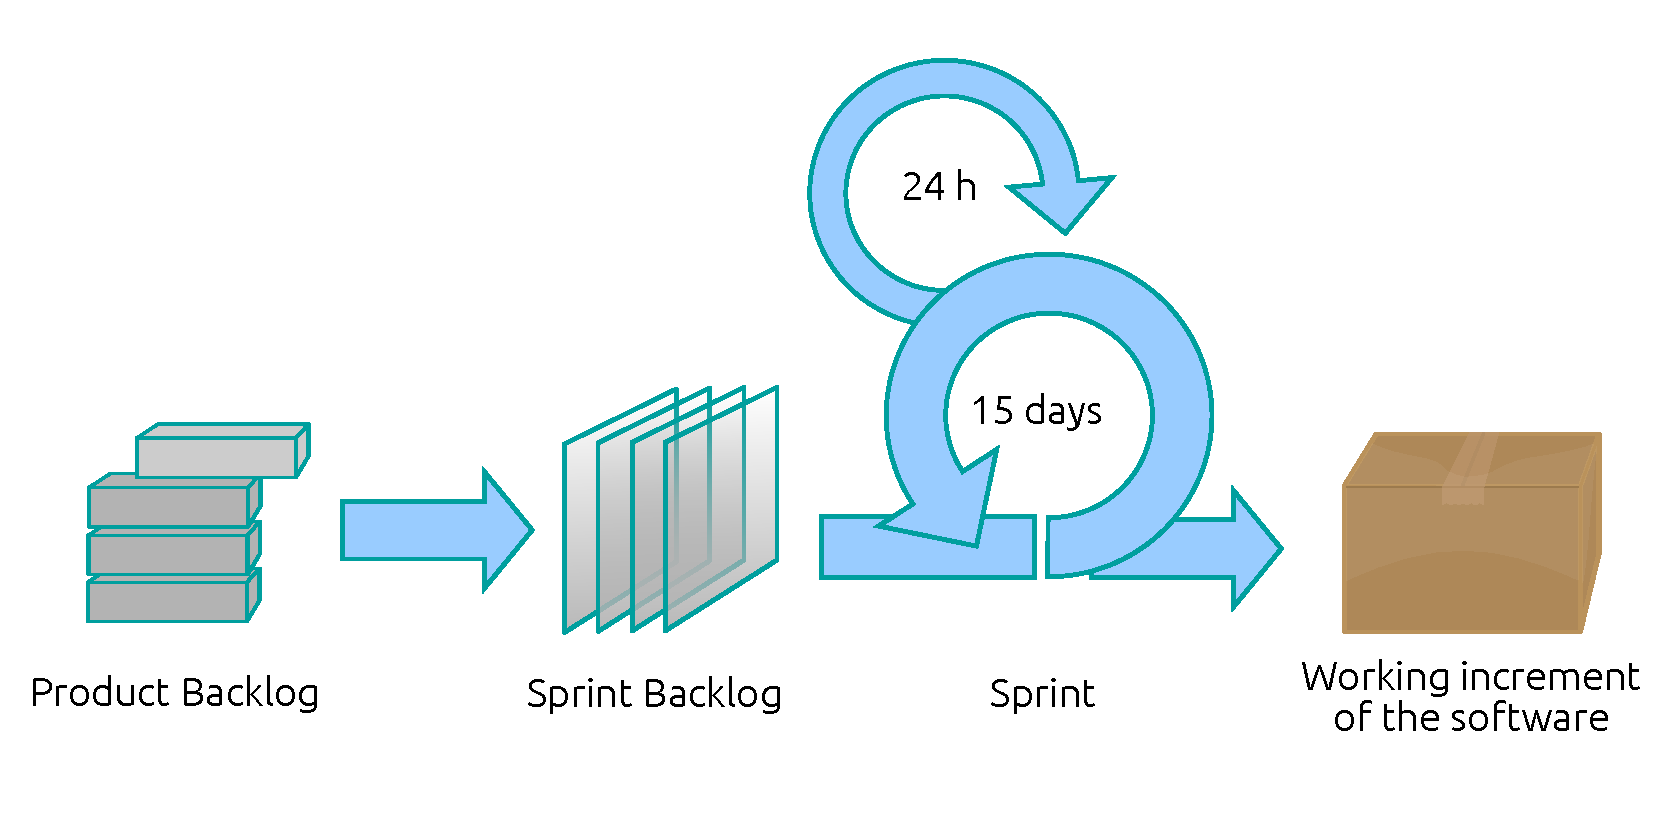
\includegraphics[width=0.8\linewidth]{figures/scrum.pdf}
	\caption[Scrum methodology workflow.]{\textit{Scrum} methodology process overview. Adapted from Wikimedia~\citep{web:Wiki:ScrumProcess}}
	\label{fig:scrum}
\end{figure}

This methodology is based on the adoption of certain roles, as well as some \textit{artifacts} and predefined processes, all of which can be adapted as necessary by the team to suit their specific needs and resources. However, a central concept forms the basis for the rest of the framework: the \textbf{sprint}. A sprint or iteration is the basic unit of development in Scrum. The sprint is a timeboxed effort, this is, it is restricted to a specific duration, which is fixed in advance for each sprint and is normally between one week and one month, with two weeks being the most common.

\subsubsection*{Roles}

The follwing are the relevant roles that emerge in a Scrum developed project:

\begin{itemize}
	\item
	\textbf{Product owner:} the product owner represents the stakeholders and is the voice of the customer. He or she is accountable for ensuring that the team delivers value to the business. The product owner writes \textit{user stories} (tasks) and adds them to the \textit{product backlog}, prioritizing them.
	
	\item
	\textbf{Scrum master:} Scrum is facilitated by a scrum master, who is accountable for removing impediments to the ability of the team to deliver the product goals and deliverables. The scrum master is not a traditional team lead or project manager, but acts as a buffer between the team and any distracting influences. The scrum master ensures that the scrum process is used as intended.
	
	\item
	\textbf{Development team:} the development team is responsible for delivering potentially shippable increments of product at the end of each \textit{sprint}. A team is made up of 3–9 individuals with cross-functional skills who do the actual work: analyse, design, develop, test, document, etc. Finally, it is important to emphasize that the development team in Scrum is self-organizing.
\end{itemize}

\subsubsection*{Events}

A series of \textit{events} take place during the Scrum process, configuring the actual workflow of the team. We will provide an overview of some of them:

\begin{itemize}
	\item
	\textbf{Sprint planning:} at the beginning of a sprint, the team holds a sprint planning event, in which the work to be done is selected from the product backlog and transferred to the sprint backlog.
	
	\item
	\textbf{Daily Scrum:} a stand-up, timeboxed and short meeting takes place every day during each sprint. In these meetings, every member of the team explains the work carried out the previous day, discusses any impediment or blocking situation he or she has encountered and decides which tasks will do in the following day.
	
	\item
	\textbf{Retrospective:} at the end of each sprint, a review of the work that has been completed is made, and the team reflects on the past sprint to identify and agree on any process improvement, which requires actions to be taken in the upcoming sprint.
\end{itemize}

\subsubsection*{Artifacts}

Even though we have given an overview of some of them, the following artifacts are the remaining pieces that shape up the Scrum process and methodology:

\begin{itemize}
	\item
	\textbf{Product backlog:} the product backlog is an ordered list of requirements that is maintained for a product. It consists of features, bug fixes, non-functional requirements, etc., i.e., whatever needs to be done in order to successfully deliver a viable product. The items in this backlog are ordered by the product owner based on considerations like risk, business value, dependencies or date needed, for example.
	
	\item
	\textbf{Sprint backlog:} The sprint backlog is the list of work the development team must address during the next sprint. The list is derived by selecting product backlog items from the top of the product backlog until the development team feels it has enough work to fill the sprint. The development team should keep in mind its past performance assessing its capacity for the new sprint, and use this as a guide line of how much \textit{effort} they can complete.
\end{itemize}

\subsection{Agile in this project}

The methodology chosen for this project will be based upon Scrum, but major modifications will have to be made, for a number of reasons. Firstly, there is no such \textit{development team}: a single developer will take care of the implementation of the project. Moreover, there is no possibility of having a Scrum master either. The project director will take a role between a technical coordinator and a product owner, although no real concept of \textit{product} exists in the project, either way.

\subsubsection{Practices}

The adopted Agile practices for this project include:

\begin{itemize}
	\item The usage of Trello\footnote{Its description, along with other resources and tools used, can be found on~\sref{Management:Budget:Resources}} as a task tracking tool, to prioritize them similarly to the Scrum backlogs.
	\item \textbf{Sprint}-based development cycles with a sprint duration of one week.
	\item Constant (re)-evaluation of constraints and requirements, to forsee changes and take preventive action (similar to retrospectives, but less formal and certainly shorter).
\end{itemize}

\subsubsection{Scope}

Adopting Agile methodologies involves several decisions on how to manage the project and its requirements. In this particular project, if we are to examine the classical constraints (of which we talked about at the beginning of this chapter), we must be aware that the \textit{schedule is fixed} (perhaps not the planning, but the final milestone) and this forces us to let the \textbf{scope opened}. This means that we will implement as much features as we can, assessing their quality, but no feature list will drive the success or failure of the project. Because we will be working on the basis of such an \textit{open scope}, deviations in this field are likely to happen. These, however, will not result in a project failure in any case, because an agreement has been reached to work this way.